\documentclass[a4paper,11pt]{article}

% Kodovani (cestiny) v dokumentu: utf-8
%\usepackage[cp1250]{inputenc}	% Omezena stredoevropska kodova stranka, pouze MSW.
\usepackage[utf8]{inputenc}	% Doporucujeme pouzivat UTF-8 (unicode).

\usepackage[margin=2cm]{geometry}
\newtoks\jmenopraktika \newtoks\jmeno \newtoks\datum
\newtoks\obor \newtoks\skupina \newtoks\rocnik \newtoks\semestr
\newtoks\cisloulohy \newtoks\jmenoulohy
\newtoks\tlak \newtoks\teplota \newtoks\vlhkost

\jmenopraktika={Fyzikální praktikum 3}
\jmeno={Lukáš Lejdar}
\datum={29. dubna 2025}
\obor={F}
\skupina={Út 14:00}

\cisloulohy={3}
\jmenoulohy={Millikanův experiment}

\tlak={101{,}35}
\teplota={21,1}
\vlhkost={47,7}


%%%%%%%%%%% Uzitecne balicky:
\usepackage[czech]{babel}

\usepackage{graphicx}
\usepackage{amsmath}
\usepackage{xspace}
\usepackage{url}
\usepackage{indentfirst}
\usepackage{wrapfig}
\usepackage{xcolor}
\usepackage{subfig}
\usepackage{subcaption}
\usepackage{enumitem}
\usepackage{tikzsymbols}
\usepackage{newfloat}

\DeclareFloatingEnvironment[fileext=lof]{graph}
\captionsetup[graph]{labelformat=simple, labelsep=colon, name=Graf}

%%%%%% Zamezeni parchantu:
\widowpenalty 10000 \clubpenalty 10000 \displaywidowpenalty 10000
%%%%%% Parametry pro moznost vsazeni vetsiho poctu obrazku na stranku
\setcounter{topnumber}{3}	  % max. pocet floatu nahore (specifikace t)
\setcounter{bottomnumber}{3}	  % max. pocet floatu dole (specifikace b)
\setcounter{totalnumber}{6}	  % max. pocet floatu na strance celkem
\renewcommand\topfraction{0.9}	  % max podil stranky pro floaty nahore
\renewcommand\bottomfraction{0.9} % max podil stranky pro floaty dole
\renewcommand\textfraction{0.1}	  % min podil stranky, ktery musi obsahovat text
\intextsep=8mm \textfloatsep=8mm  %\intextsep pro ulozeni [h] floatu a \textfloatsep pro [b] or [t]

% Tecky za cisly sekci:
\renewcommand{\thesection}{\arabic{section}.}
\renewcommand{\thesubsection}{\thesection\arabic{subsection}.}
% Jednopismenna mezera mezi cislem a nazvem kapitoly:
\makeatletter \def\@seccntformat#1{\csname the#1\endcsname\hspace{1ex}} \makeatother
%
\newcommand{\vsn}[4]{\ensuremath{#1 =} #2(#3)\,#4}
\newcommand{\vrn}[6]{\ensuremath{#1 =} (#2 $\pm$ #3)\,#4 ($p=$ #5\,\%, $\nu=$ #6)}

\newcommand*\circled[1]{\tikz[baseline=(char.base)]{
		\node[shape=circle,draw,inner sep=1pt] (char) {#1};}}

%%%%%%%%%%%%%%%%%%%%%%%%%%%%%%%%%%%%%%%%%%%%%%%%%%%%%%%%%%%%%%%%%%%%%%%%%%%%%%%
% Zacatek dokumentu
%%%%%%%%%%%%%%%%%%%%%%%%%%%%%%%%%%%%%%%%%%%%%%%%%%%%%%%%%%%%%%%%%%%%%%%%%%%%%%%

\usepackage{listings}

\definecolor{codegray}{gray}{0.95}

\lstdefinestyle{mypython}{
    backgroundcolor=\color{codegray},
    language=Python,
    basicstyle=\ttfamily\footnotesize,
    keywordstyle=\color{blue},
    commentstyle=\color{green!60!black},
    stringstyle=\color{orange},
    showstringspaces=false,
    breaklines=true,
    tabsize=4
}

\begin{document}

\thispagestyle{empty}

{
\begin{center}
\sf 
{\Large Ústav fyziky a technologií plazmatu Přírodovědecké fakulty Masarykovy univerzity} \\
\bigskip
{\huge \bfseries FYZIKÁLNÍ PRAKTIKUM} \\
\bigskip
{\Large \the\jmenopraktika}
\end{center}

\bigskip

\sf
\noindent
\setlength{\arrayrulewidth}{1pt}
\begin{tabular*}{\textwidth}{@{\extracolsep{\fill}} l l}
\large {\bfseries Zpracoval:}  \the\jmeno & \large  {\bfseries Naměřeno:} \the\datum\\[2mm]
\large  {\bfseries Obor:} \the\obor  \hspace{40mm}  {\bfseries Skupina:} \the\skupina %
&\large {\bfseries Testováno:}\\
\\
\hline
\end{tabular*}
}

\bigskip

{
\sf
\noindent \begin{tabular}{p{4cm} p{0.6\textwidth}}
\Large  Úloha č. {\bfseries \the\cisloulohy:} \par
\smallskip
&\Large \bfseries \the\jmenoulohy  \\[2mm]
\end{tabular}
}

\vspace{-10pt}

\section{Úvod}

V této úloze budu měřit náboje malých olejových kapiček. Ukáže se, že tyto náboje jsou celočíselnými násobky elementárního náboje, který je pak možné vypočítat. Tento experiment poprvé provedl Robert A. Millikan v roce 1913, za který později dostal Nobelovu cenu za Fyziku.

\section{Teorie}

Principem Millikanova experimentu je měření rovnovážné rychlosti kapičky oleje. Síla působící na takovou kapičku v důsledku intenzity elektrického pole $ E $ bude

\begin{equation}
F_e =  \mid q \mid E
\end{equation}

\noindent
kde $ q $ je náboj kapičky. Mimo to bude uvnitř měřící komory působit několik dalších sil, které je potřeba započíst. První z nich je gravitační síla

\begin{equation}
F_g = \frac{4}{3} \pi r^{3} \rho g
\end{equation}

\noindent
kde $ r $ je poloměr kapičky, $ \rho $ je hustota oleje a $ g $ je tíhové zrychlení. Potom vztlaková síla

\begin{equation}
F_{vz} =  \frac{4}{3} \pi r^{3} \rho_{vz} g
\end{equation}

\noindent
kde $ \rho_{vz} $ je hustota vzduchu a odporová síla vyjádřená Stokesovým zákonem

\begin{equation}
 F_t = 6 \pi \eta r v
\end{equation}

\noindent
kde $ \eta $ je viskozita vzduchu a $ v $ rychlosti kapičky. Síla elektrického pole bude v experimentálním uspořádání působit buď směrem proti gravitačnímu zrychlení nebo s ním. Pokud naměříme rovnovážnou rychlost jedné kapičky v obou případech, dostaneme dvě rovnice o neznámých $ r $ a $ q $ 

\begin{align*}
    \frac{4}{3} \pi r^{3} \rho g + 6 \pi \eta r v_1 = | q |  E + \frac{4}{3} \pi r^{3} \rho_{vz} g \\
    \frac{4}{3} \pi r^{3} \rho g + 6 \pi \eta r v_2  + | q |  E = \frac{4}{3} \pi r^{3} \rho_{vz} g
\end{align*}

\noindent
které z nich vyjádříme jako

\begin{equation}
r^2 = \frac{9 \eta (v_1 - v_2) }{4 g (\rho - \rho_{vz})}
\end{equation}

\begin{equation}
|q| = 3 \pi \eta r \frac{v_1 + v_2}{E}
\end{equation}

\section{Postup měření}

Fotka měřící aparatury je na Obrázku (1). Základem je komůrka s kondenzátorem kam se  vstřikují olejové kapičky ze skleněné nádoby pomocí gumového balónku. Některé kapky se při vstřikování nabíjejí třením, další mohou získat náboj díky připojenému zdroji $ \alpha $-částic  ($ ^{241} $Am, 74 kBq ).

Komůrka je vybavená vodováhou, osvětlovací lampou a mikroskopem pro sledování kapek. Napětí na kondenzátoru zajišťuje zdroj regulovatelného napětí v rozmezí (0-300V) a druhý zdroj zapojený do série s prvním o fixním napětí (300V). Sledovat pohyb kapek umožňuje kamera skrz zvětšovací objektiv. 

\begin{figure}[htpb]
    \centering
    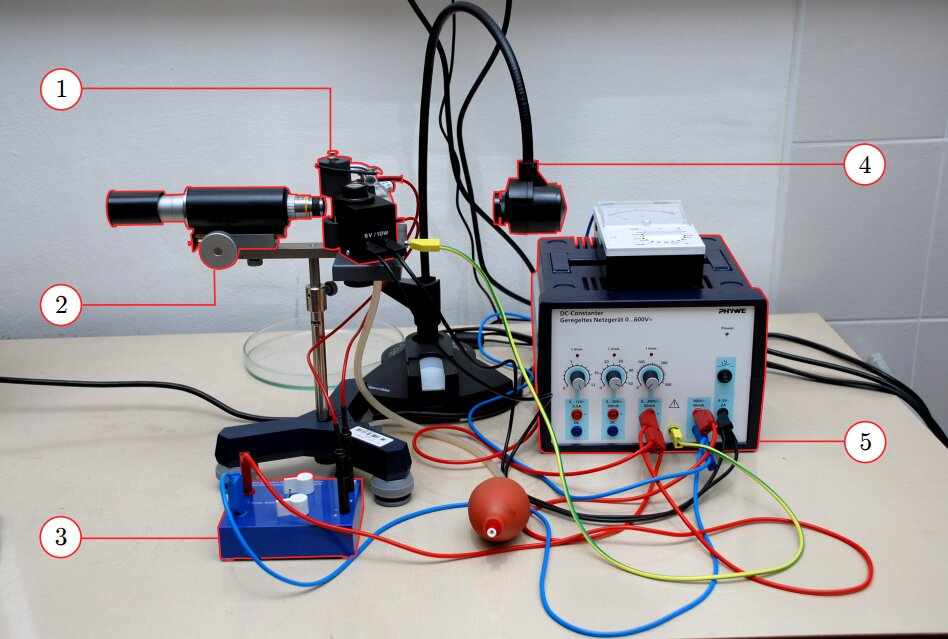
\includegraphics[width=0.6\textwidth]{aparatura.jpg}
    \caption{Zapojení aparatury, 1 - komůrka s kondenzátorem, 2 - mikroskop, 3 - přepínač napětí, 4 - kamera, 5 - zdroj napětí}
\end{figure}

\section{Zpracování měření}

Celkem jsem nahrál 2 až 3 videa pro každé napětí na kondenzátoru v rozmezí (300 - 600) V po 50 Voltech. Prvním krokem při zpracování je zjistit náboj alespoň 50 kapiček z jejich rychlostí před a po změně polarity napětí. Z videí bylo potřeba nejdřív digitálně odstranit pozadí a potom v každém obrázku rozpoznat kapičky. Pro tento účel existuje v pythonu knihovna trackpy, která pomocí funkce \texttt{trackpy.locate} dokáže kapičky v každém framu najít a označit. Proces zpracování jednoho framu je uvedený na Obrázcích 2.

%\begin{lstlisting}[style=mypython]
%features = trackpy.locate(gray, diameter=13, minmass=10)
%\end{lstlisting}

\begin{table}[htpb]
    \begin{minipage}{.3\linewidth}
        \centering
        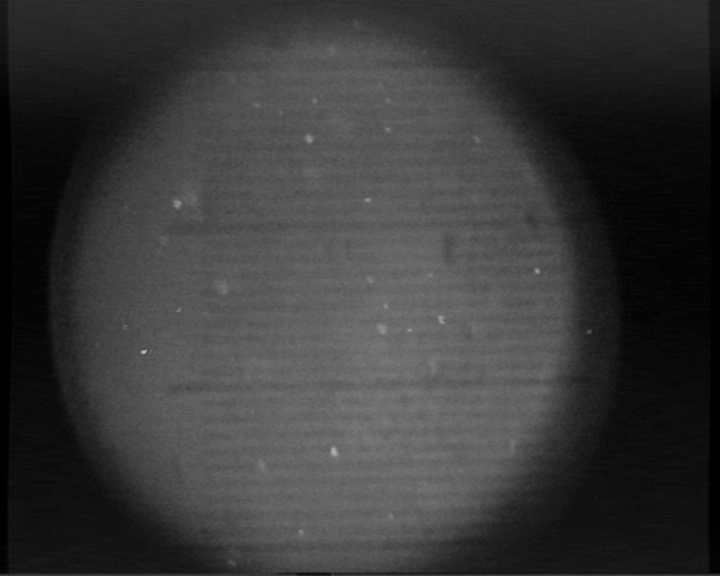
\includegraphics[width=\textwidth]{frame_o.jpg}
    \end{minipage} 
    \hfill
    \begin{minipage}{.3\linewidth}
        \centering
        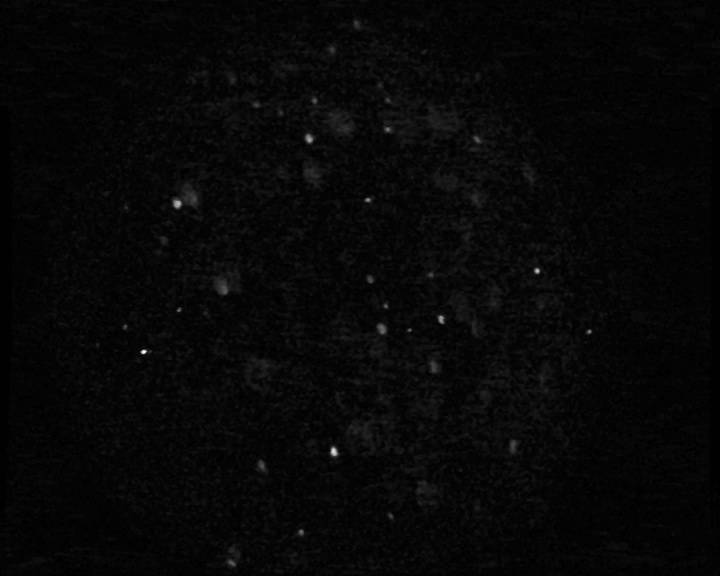
\includegraphics[width=\textwidth]{frame_bc.jpg}
    \end{minipage} 
    \hfill
    \begin{minipage}{.3\linewidth}
        \centering
        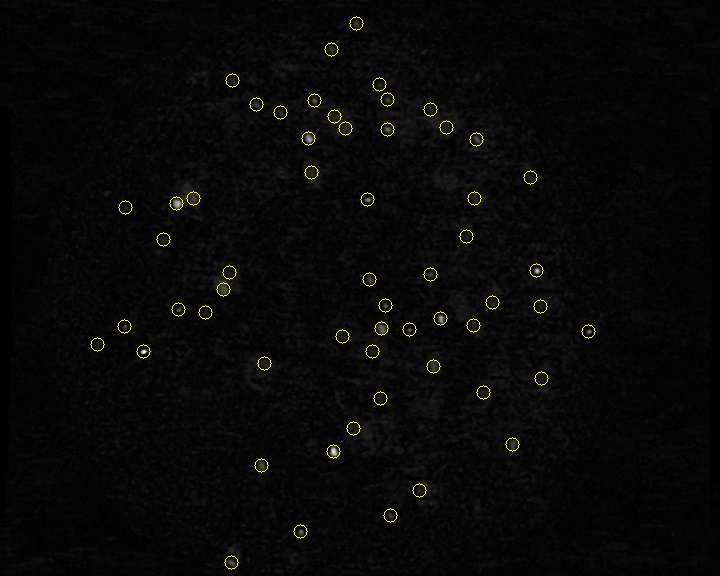
\includegraphics[width=\textwidth]{frame_f.jpg}
    \end{minipage} 
    \hfill
    \captionsetup{type=figure}
    \caption{Postup zpracování každého framu z videa. Nalevo je vidět původní obrázek, uprostřed bylo odebrané pozadí a napravo je jsou anotované rozpoznané kapičky. }
\end{table}

Rozpoznání kapek v každém jednotlivém framu ještě neumožňuje určit, která kapička odpovídá které v následujícím framu. K propojení těchto bodů do trajektorií napříč framy souží v knihovně funkce \texttt{trackpy.link}. V Grafu 3 je uveden příklad zpracovaného videa při napětí 300 V. 

\begin{figure}[htpb]
    \centering
    % GNUPLOT: LaTeX picture with Postscript
\begingroup
  \makeatletter
  \providecommand\color[2][]{%
    \GenericError{(gnuplot) \space\space\space\@spaces}{%
      Package color not loaded in conjunction with
      terminal option `colourtext'%
    }{See the gnuplot documentation for explanation.%
    }{Either use 'blacktext' in gnuplot or load the package
      color.sty in LaTeX.}%
    \renewcommand\color[2][]{}%
  }%
  \providecommand\includegraphics[2][]{%
    \GenericError{(gnuplot) \space\space\space\@spaces}{%
      Package graphicx or graphics not loaded%
    }{See the gnuplot documentation for explanation.%
    }{The gnuplot epslatex terminal needs graphicx.sty or graphics.sty.}%
    \renewcommand\includegraphics[2][]{}%
  }%
  \providecommand\rotatebox[2]{#2}%
  \@ifundefined{ifGPcolor}{%
    \newif\ifGPcolor
    \GPcolorfalse
  }{}%
  \@ifundefined{ifGPblacktext}{%
    \newif\ifGPblacktext
    \GPblacktexttrue
  }{}%
  % define a \g@addto@macro without @ in the name:
  \let\gplgaddtomacro\g@addto@macro
  % define empty templates for all commands taking text:
  \gdef\gplbacktext{}%
  \gdef\gplfronttext{}%
  \makeatother
  \ifGPblacktext
    % no textcolor at all
    \def\colorrgb#1{}%
    \def\colorgray#1{}%
  \else
    % gray or color?
    \ifGPcolor
      \def\colorrgb#1{\color[rgb]{#1}}%
      \def\colorgray#1{\color[gray]{#1}}%
      \expandafter\def\csname LTw\endcsname{\color{white}}%
      \expandafter\def\csname LTb\endcsname{\color{black}}%
      \expandafter\def\csname LTa\endcsname{\color{black}}%
      \expandafter\def\csname LT0\endcsname{\color[rgb]{1,0,0}}%
      \expandafter\def\csname LT1\endcsname{\color[rgb]{0,1,0}}%
      \expandafter\def\csname LT2\endcsname{\color[rgb]{0,0,1}}%
      \expandafter\def\csname LT3\endcsname{\color[rgb]{1,0,1}}%
      \expandafter\def\csname LT4\endcsname{\color[rgb]{0,1,1}}%
      \expandafter\def\csname LT5\endcsname{\color[rgb]{1,1,0}}%
      \expandafter\def\csname LT6\endcsname{\color[rgb]{0,0,0}}%
      \expandafter\def\csname LT7\endcsname{\color[rgb]{1,0.3,0}}%
      \expandafter\def\csname LT8\endcsname{\color[rgb]{0.5,0.5,0.5}}%
    \else
      % gray
      \def\colorrgb#1{\color{black}}%
      \def\colorgray#1{\color[gray]{#1}}%
      \expandafter\def\csname LTw\endcsname{\color{white}}%
      \expandafter\def\csname LTb\endcsname{\color{black}}%
      \expandafter\def\csname LTa\endcsname{\color{black}}%
      \expandafter\def\csname LT0\endcsname{\color{black}}%
      \expandafter\def\csname LT1\endcsname{\color{black}}%
      \expandafter\def\csname LT2\endcsname{\color{black}}%
      \expandafter\def\csname LT3\endcsname{\color{black}}%
      \expandafter\def\csname LT4\endcsname{\color{black}}%
      \expandafter\def\csname LT5\endcsname{\color{black}}%
      \expandafter\def\csname LT6\endcsname{\color{black}}%
      \expandafter\def\csname LT7\endcsname{\color{black}}%
      \expandafter\def\csname LT8\endcsname{\color{black}}%
    \fi
  \fi
    \setlength{\unitlength}{0.0500bp}%
    \ifx\gptboxheight\undefined%
      \newlength{\gptboxheight}%
      \newlength{\gptboxwidth}%
      \newsavebox{\gptboxtext}%
    \fi%
    \setlength{\fboxrule}{0.5pt}%
    \setlength{\fboxsep}{1pt}%
    \definecolor{tbcol}{rgb}{1,1,1}%
\begin{picture}(6048.00,3600.00)%
    \gplgaddtomacro\gplbacktext{%
      \csname LTb\endcsname%%
      \put(814,704){\makebox(0,0)[r]{\strut{}$0$}}%
      \put(814,1150){\makebox(0,0)[r]{\strut{}$100$}}%
      \put(814,1596){\makebox(0,0)[r]{\strut{}$200$}}%
      \put(814,2042){\makebox(0,0)[r]{\strut{}$300$}}%
      \put(814,2487){\makebox(0,0)[r]{\strut{}$400$}}%
      \put(814,2933){\makebox(0,0)[r]{\strut{}$500$}}%
      \put(814,3379){\makebox(0,0)[r]{\strut{}$600$}}%
      \put(946,484){\makebox(0,0){\strut{}$0$}}%
      \put(1618,484){\makebox(0,0){\strut{}$50$}}%
      \put(2290,484){\makebox(0,0){\strut{}$100$}}%
      \put(2962,484){\makebox(0,0){\strut{}$150$}}%
      \put(3635,484){\makebox(0,0){\strut{}$200$}}%
      \put(4307,484){\makebox(0,0){\strut{}$250$}}%
      \put(4979,484){\makebox(0,0){\strut{}$300$}}%
      \put(5651,484){\makebox(0,0){\strut{}$350$}}%
    }%
    \gplgaddtomacro\gplfronttext{%
      \csname LTb\endcsname%%
      \put(209,2041){\rotatebox{-270}{\makebox(0,0){\strut{}$ y $ (px)}}}%
      \put(3298,154){\makebox(0,0){\strut{}$ t $ (frame)}}%
    }%
    \gplbacktext
    \put(0,0){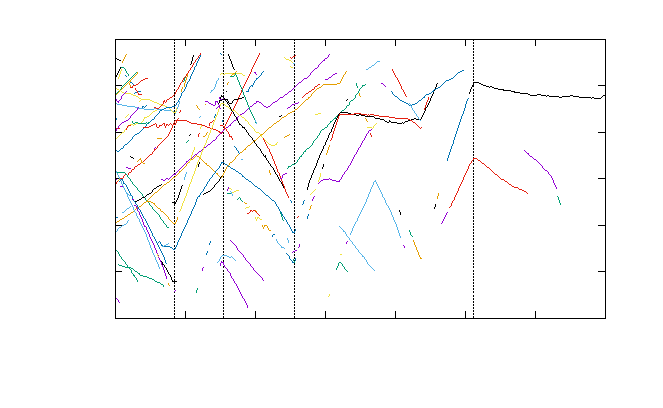
\includegraphics[width={302.40bp},height={180.00bp}]{traj}}%
    \gplfronttext
  \end{picture}%
\endgroup

    \captionsetup{type=graph}
    \caption{Trajektorie kapiček při napětí 300 V}
\end{figure}

V obrázku jsou jasně rozpoznatelné místa, kde několik kapek ostře změní směr letu, kvůli změně polarity napětí. Z trajektorií jsem vybíral jen ty, které jsou co nejpřímější před a po změně napětí a z lineárního fitu určil jejich rychlosti $ v_1 $ a $ v_2 $. Tímto způsobem jsem z 15 videí získal 61 měření a podle vztahů (5) a (6) vypočítal výsledné náboje. Tyto náboje jsou ve vzestupném pořadí vykreslené do Grafu 2.

\begin{figure}[htpb]
    \centering
    % GNUPLOT: LaTeX picture with Postscript
\begingroup
  \makeatletter
  \providecommand\color[2][]{%
    \GenericError{(gnuplot) \space\space\space\@spaces}{%
      Package color not loaded in conjunction with
      terminal option `colourtext'%
    }{See the gnuplot documentation for explanation.%
    }{Either use 'blacktext' in gnuplot or load the package
      color.sty in LaTeX.}%
    \renewcommand\color[2][]{}%
  }%
  \providecommand\includegraphics[2][]{%
    \GenericError{(gnuplot) \space\space\space\@spaces}{%
      Package graphicx or graphics not loaded%
    }{See the gnuplot documentation for explanation.%
    }{The gnuplot epslatex terminal needs graphicx.sty or graphics.sty.}%
    \renewcommand\includegraphics[2][]{}%
  }%
  \providecommand\rotatebox[2]{#2}%
  \@ifundefined{ifGPcolor}{%
    \newif\ifGPcolor
    \GPcolorfalse
  }{}%
  \@ifundefined{ifGPblacktext}{%
    \newif\ifGPblacktext
    \GPblacktexttrue
  }{}%
  % define a \g@addto@macro without @ in the name:
  \let\gplgaddtomacro\g@addto@macro
  % define empty templates for all commands taking text:
  \gdef\gplbacktext{}%
  \gdef\gplfronttext{}%
  \makeatother
  \ifGPblacktext
    % no textcolor at all
    \def\colorrgb#1{}%
    \def\colorgray#1{}%
  \else
    % gray or color?
    \ifGPcolor
      \def\colorrgb#1{\color[rgb]{#1}}%
      \def\colorgray#1{\color[gray]{#1}}%
      \expandafter\def\csname LTw\endcsname{\color{white}}%
      \expandafter\def\csname LTb\endcsname{\color{black}}%
      \expandafter\def\csname LTa\endcsname{\color{black}}%
      \expandafter\def\csname LT0\endcsname{\color[rgb]{1,0,0}}%
      \expandafter\def\csname LT1\endcsname{\color[rgb]{0,1,0}}%
      \expandafter\def\csname LT2\endcsname{\color[rgb]{0,0,1}}%
      \expandafter\def\csname LT3\endcsname{\color[rgb]{1,0,1}}%
      \expandafter\def\csname LT4\endcsname{\color[rgb]{0,1,1}}%
      \expandafter\def\csname LT5\endcsname{\color[rgb]{1,1,0}}%
      \expandafter\def\csname LT6\endcsname{\color[rgb]{0,0,0}}%
      \expandafter\def\csname LT7\endcsname{\color[rgb]{1,0.3,0}}%
      \expandafter\def\csname LT8\endcsname{\color[rgb]{0.5,0.5,0.5}}%
    \else
      % gray
      \def\colorrgb#1{\color{black}}%
      \def\colorgray#1{\color[gray]{#1}}%
      \expandafter\def\csname LTw\endcsname{\color{white}}%
      \expandafter\def\csname LTb\endcsname{\color{black}}%
      \expandafter\def\csname LTa\endcsname{\color{black}}%
      \expandafter\def\csname LT0\endcsname{\color{black}}%
      \expandafter\def\csname LT1\endcsname{\color{black}}%
      \expandafter\def\csname LT2\endcsname{\color{black}}%
      \expandafter\def\csname LT3\endcsname{\color{black}}%
      \expandafter\def\csname LT4\endcsname{\color{black}}%
      \expandafter\def\csname LT5\endcsname{\color{black}}%
      \expandafter\def\csname LT6\endcsname{\color{black}}%
      \expandafter\def\csname LT7\endcsname{\color{black}}%
      \expandafter\def\csname LT8\endcsname{\color{black}}%
    \fi
  \fi
    \setlength{\unitlength}{0.0500bp}%
    \ifx\gptboxheight\undefined%
      \newlength{\gptboxheight}%
      \newlength{\gptboxwidth}%
      \newsavebox{\gptboxtext}%
    \fi%
    \setlength{\fboxrule}{0.5pt}%
    \setlength{\fboxsep}{1pt}%
    \definecolor{tbcol}{rgb}{1,1,1}%
\begin{picture}(6336.00,3600.00)%
    \gplgaddtomacro\gplbacktext{%
      \csname LTb\endcsname%%
      \put(550,704){\makebox(0,0)[r]{\strut{}$0$}}%
      \put(550,1086){\makebox(0,0)[r]{\strut{}$1$}}%
      \put(550,1468){\makebox(0,0)[r]{\strut{}$2$}}%
      \put(550,1850){\makebox(0,0)[r]{\strut{}$3$}}%
      \put(550,2233){\makebox(0,0)[r]{\strut{}$4$}}%
      \put(550,2615){\makebox(0,0)[r]{\strut{}$5$}}%
      \put(550,2997){\makebox(0,0)[r]{\strut{}$6$}}%
      \put(550,3379){\makebox(0,0)[r]{\strut{}$7$}}%
      \put(682,484){\makebox(0,0){\strut{}$0$}}%
      \put(1379,484){\makebox(0,0){\strut{}$10$}}%
      \put(2076,484){\makebox(0,0){\strut{}$20$}}%
      \put(2773,484){\makebox(0,0){\strut{}$30$}}%
      \put(3470,484){\makebox(0,0){\strut{}$40$}}%
      \put(4167,484){\makebox(0,0){\strut{}$50$}}%
      \put(4865,484){\makebox(0,0){\strut{}$60$}}%
    }%
    \gplgaddtomacro\gplfronttext{%
      \csname LTb\endcsname%%
      \put(209,2041){\rotatebox{-270}{\makebox(0,0){\strut{}$ q \cdot 10^{-19}$ (C)}}}%
      \put(2843,154){\makebox(0,0){\strut{} měření }}%
      \csname LTb\endcsname%%
      \put(5460,895){\makebox(0,0)[l]{\strut{}300}}%
      \put(5460,1277){\makebox(0,0)[l]{\strut{}350}}%
      \put(5460,1659){\makebox(0,0)[l]{\strut{}400}}%
      \put(5460,2041){\makebox(0,0)[l]{\strut{}450}}%
      \put(5460,2423){\makebox(0,0)[l]{\strut{}500}}%
      \put(5460,2805){\makebox(0,0)[l]{\strut{}550}}%
      \put(5460,3187){\makebox(0,0)[l]{\strut{}600}}%
      \put(6186,2041){\rotatebox{-270}{\makebox(0,0){\strut{}Napětí (V)}}}%
    }%
    \gplbacktext
    \put(0,0){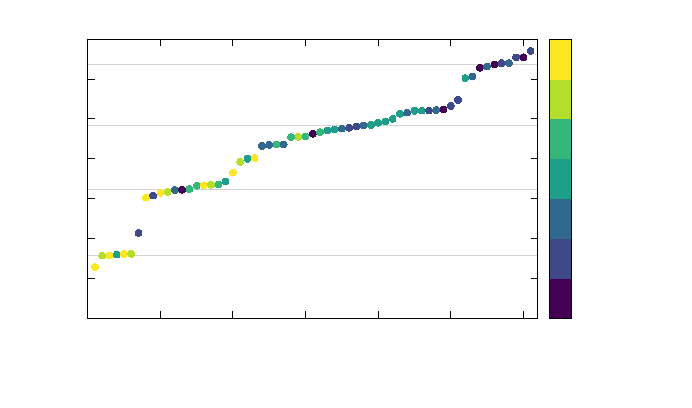
\includegraphics[width={316.80bp},height={180.00bp}]{all_charges}}%
    \gplfronttext
  \end{picture}%
\endgroup

    \captionsetup{type=graph}
    \caption{Zjištěné náboje kapiček, označené barevně podle napětí při kterých byli měřené.}
\end{figure}

Graf má spíš schodovitý charakter než spojitý průběh přímky. Některé body ale schodovitý tvar narušují, takže je vyřadím jako chybné měření. Zbylé hodnoty jsem rozdělil do skupiny a pro každou určil střední hodnotu, které vyšly postupně $ \bar{q}_1 = 1.58 $, $ \bar{q}_2 = 3.23 $, $ \bar{q}_3 = 4.84 $ a $ \bar{q}_3 = 6.36 $ v jednotkách $ 10 ^{-19} $ C. Krok mezi skupinami je přibližně 1.6, což naznačuje, že jednotlivé skupiny odpovídají celým násobkům elemntárního náboje od 1 do 4. Každé hodnotě jsem tedy přiřadil počet elementárních nábojů a získal hodnoty $ e_i = \frac{q_i}{n} $. Statistickým vyhodnocením pak vyšla konečná hodnota náboje

\begin{equation}
e = (1.61 \pm 0.03) \cdot 10^{-19} \text{ C } \ (p= 99\,\%, \nu= 52)
\end{equation}

\section{Závěr}

Změřil jsem rovnovážnou rychlost 60 kapiček při různých polaritách napětí v komoře a podle vztahů (5) a (6) potom určil jejich náboj. Ukázalo se, že náboje spadaly do rovnoměrně oddělených diskrétních hodnot, odpovídajících počtu nábojů v kapičkách. Z těchto dat už bylo možné vypočítat elementární náboj $ e = (1.61 \pm 0.03) \cdot 10^{-19} \text{ C } $. Tabulková hodnota je $ e = 1.602 \cdot 10 ^{-19} $. Největším zdrojem nejistoty je pravděpodobně výběr měřených kapiček. Nejlépe vycházejí ty, které letí rovnoměrně přímo dolů a pak nahoru, ale takových je v natočených videích málo. 

\begin{thebibliography}{0}
\bibitem{tabulky} Návod k úloze ~\url{https://is.muni.cz/auth/el/sci/jaro2025/F4210/um/fp3-3_Millikan.pdf}.   
\end{thebibliography}

\end{document}
